\documentclass{article}

\usepackage{arxiv}

\usepackage[utf8]{inputenc} % allow utf-8 input
\usepackage[T1]{fontenc}    % use 8-bit T1 fonts
\usepackage{hyperref}       % hyperlinks
\usepackage{url}            % simple URL typesetting
\usepackage{booktabs}       % professional-quality tables
\usepackage{amsfonts}       % blackboard math symbols
\usepackage{nicefrac}       % compact symbols for 1/2, etc.
\usepackage{microtype}      % microtypography
\usepackage{amsmath}
\usepackage{amssymb}
\usepackage{graphicx}
\usepackage{float}
\usepackage{appendix}

\usepackage{listings}
\usepackage{xcolor}

\definecolor{codegreen}{rgb}{0,0.6,0}
\definecolor{codegray}{rgb}{0.5,0.5,0.5}
\definecolor{codepurple}{rgb}{0.58,0,0.82}
\definecolor{backcolour}{rgb}{0.95,0.95,0.92}

\lstdefinestyle{mystyle}{
    backgroundcolor=\color{backcolour},   
    commentstyle=\color{codegreen},
    keywordstyle=\color{magenta},
    numberstyle=\tiny\color{codegray},
    stringstyle=\color{codepurple},
    basicstyle=\ttfamily\footnotesize,
    breakatwhitespace=false,         
    breaklines=true,                 
    captionpos=b,                    
    keepspaces=true,                 
    numbers=left,                    
    numbersep=5pt,                  
    showspaces=false,                
    showstringspaces=false,
    showtabs=false,                  
    tabsize=2
}

\lstset{style=mystyle}

\title{ME 250H Project1}

\author{
  Ziheng ~Ge \\
  UID: 805221224 \\
  Department of Mathematics\\
  UCLA\\
}

\begin{document}
\maketitle

\begin{abstract}
In this project I practiced several finite difference schemes using Python. In problem 1 I applied central difference scheme and midpoint difference scheme to calculate derivative of Bessel function $J_0(x)$. I also verified their order of accuracy. In problem 2, I numerically solved advection equation with several time stepping methods and finite difference schemes. We observed dispersive error in central difference scheme, and diffusive error in upwind difference scheme.
\end{abstract}

\section{Problem 1}
    Bessel function $J_0(x)$ is implemented in scipy.special. As we know
    $$J_0'(x)=-J_1(x)$$
    Here we plot them with $x\in [0,20], dx=0.1$
    \begin{figure}[H]
        \centering
        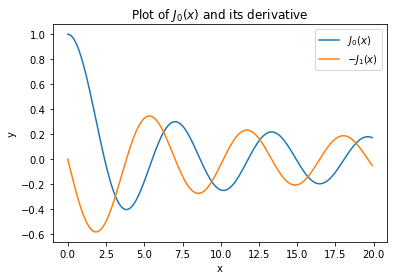
\includegraphics[width = 8cm]{pictures/pic1.png}
    \end{figure}
\subsection{Central difference scheme}
First, we define a function for central difference scheme. We calculate the derivatives at grid nodes.
\begin{itemize}
    \item Order 2:
    $$f'(x_j)=\frac{-f_{j-1} + f_{j+1}}{2\Delta x}$$
    \item Order 4:
    $$f'(x_j)=\frac{f_{j-2} - 8f_{j-1} + 8f_{j+1} - f_{j+2}}{12\Delta x}$$
\end{itemize}
We abandon the boundary nodes that we cannot directly get from the central schemes. Although there are one sided difference schemes of the same order, we don't know how it affects the order of total error. Also, in practice we have certain boundary conditions that we should analyze the error separately.

Now we apply the central difference scheme on Bessel function $J_0(x)$, and compare with the accurate derivative $-J_1(x)$.

\begin{figure}[H]
    \centering
    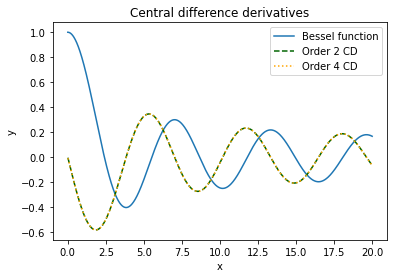
\includegraphics[width = 8cm]{pictures/pic2.png}
\end{figure}

We can see it's almost identical. To measure the order of accuracy for the schemes, we calculate the RMSE (Root Mean Squared Error), which is same as 2-norm or the error. Here we plot $\log(err)$ against $\log(dx)$, dx shrink by half for each calculation.

\begin{figure}[H]
    \centering
    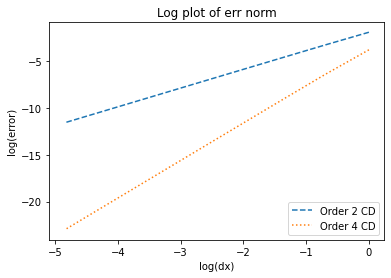
\includegraphics[width = 8cm]{pictures/pic3.png}
\end{figure}

Order of accuracy $\alpha$ means 
$$err\sim Cdx^\alpha\ \Rightarrow\  \log(err)=\log(dx)+\tilde{C}$$ 
Therefore the order can be approximated by the slope of log plot. Here we can observe that the orders are about 2 and 4, as we expected.

\subsection{Mid-point difference scheme}
First, we define a function for mid-point difference scheme. Different from central scheme, we calculate the derivatives at mid-point nodes $x_{j+1/2}$.
\begin{itemize}
    \item Order 2:
    $$f'(x_j)=\frac{-f_{j-1/2} + f_{j+1/2}}{\Delta x}$$
    \item Order 4:
    $$f'(x_j)=\frac{f_{j-3/2} - 27f_{j-1/2} + 27f_{j+1/2} - f_{j+3/2}}{24\Delta x}$$
\end{itemize}
Similar to central schemes, we abandon the boundary nodes that we cannot directly get from mid-point scheme, to avoid extra errors. Now we apply the mid-point scheme on Bessel function $J_0(x)$, and compare with the accurate derivative $-J_1(x)$.

\begin{figure}[H]
    \centering
    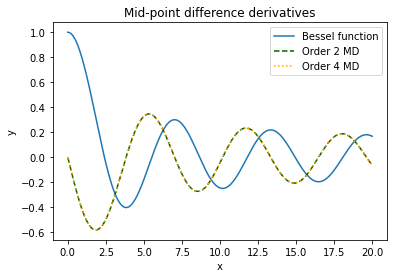
\includegraphics[width = 8cm]{pictures/pic4.png}
\end{figure}

We also plot the log of RMSE against $\log(dx)$, dx shrink by half for each calculation.

\begin{figure}[H]
    \centering
    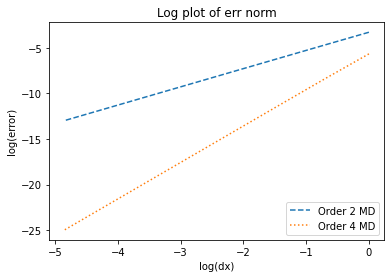
\includegraphics[width = 8cm]{pictures/pic5.png}
\end{figure}

From the slope of plot, we can observe that the orders are about 2 and 4, as we expected.

\section{Problem 2}
Numerically solve the advection equation
$$\frac{\partial f}{\partial x} + \frac{\partial f}{\partial t} = 0,\hspace{3mm} (x,t)\in[0,5]\times[0,3]$$
With initial condition
$$f(0,x) = \begin{cases}
1 & 1\leqslant x\leqslant 2 \\
2 & otherwise
\end{cases}$$
Here use forward Euler method and predictor-corrector method (RK2) for time stepping. We use central scheme and upwind scheme for finite differencing.

\subsection{Forward Euler method}
We first try forward Euler method.
\begin{itemize}
\item Central difference scheme:
$$f_j^{n+1}=f_j^n-\frac{\Delta t}{2\Delta x}(f_{j+1}^n-f_{j-1}^n)$$
\item Upwind difference scheme:
$$f_j^{n+1}=f_j^n-\frac{\Delta t}{\Delta x}(f_{j}^n-f_{j-1}^n)$$
It's called "upwind" because the traveling of information is consistent with the characteristic of this ODE 
$$x-t=const$$
\end{itemize}
We assume periodic boundary condition, i.e. frictional nodes
$$f_M=f_0,\ f_{-1}=f_{M-1}$$
Now we set $dx=0.1, dt=0.01$, and from the two schemes we get the following plot of solution
\begin{figure}[H]
    \centering
    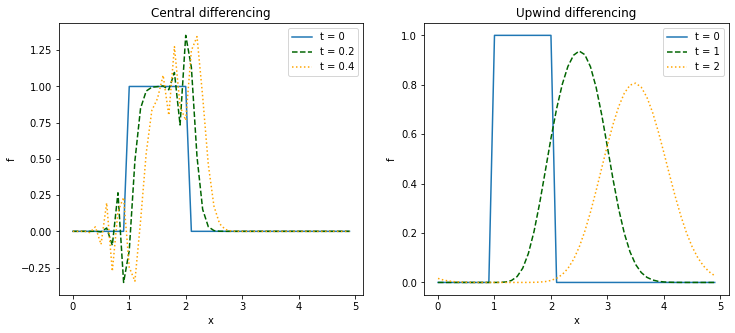
\includegraphics[width = 15cm]{pictures/pic6.png}
\end{figure}
We can observe the dispersive error in central scheme and diffusive error in upwind scheme, as shown in Fig. 2.13 in our textbook \cite{kajishima2017computational}.

\subsection{Predictor-correcter method (RK2)}
Now we try the 2nd Runge-Kutta method (RK2), which is expected to be more accurate than forward Euler method.

\begin{itemize}
\item Central difference scheme:
First calculate prediction
$$f_j^*=f_j^n-\frac{\Delta t}{4\Delta x}(f_{j+1}^n-f_{j-1}^n)$$
Then calculate correction
$$f_j^{n+1}=f_j^n-\frac{\Delta t}{2\Delta x}(f_{j+1}^*-f_{j-1}^*)$$
\item Upwind difference scheme:
First calculate prediction
$$f_j^*=f_j^n-\frac{\Delta t}{2\Delta x}(f_{j}^n-f_{j-1}^n)$$
Then calculate correction
$$f_j^{n+1}=f_j^n-\frac{\Delta t}{\Delta x}(f_{j}^*-f_{j-1}^*)$$
\end{itemize}
Now we set $dx=0.1, dt=0.01$, and from the two schemes we get the following plot of solution
\begin{figure}[H]
    \centering
    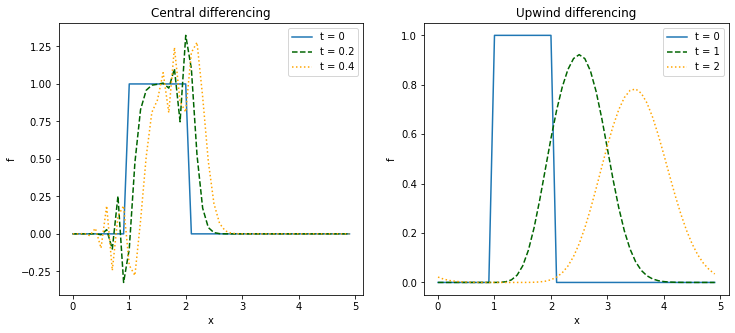
\includegraphics[width = 15cm]{pictures/pic7.png}
\end{figure}
We can observe the same dispersive and diffusive behavior as the forward Euler method. Although RK2 is expected 2nd order accurate for time, we cannot observe any difference directly from the plot of solution.

\bibliographystyle{unsrt}
\bibliography{references}

\newpage
\appendix
Here we attach part of the code for this project.
\section{Python code for Problem 1}
Central difference scheme:
\begin{lstlisting}[language = Python]
def centdiff(dx, y_data, order = 2):
## dx: grid spacing, y_data: input function, order: 2 or 4

    N = y_data.shape[0];
    
    ## 2nd order central difference
    if order == 2:
        y_deriv = np.zeros(N-2);
        for i in range(N-2):
            y_deriv[i] = (-y_data[i] + y_data[i+2]) / (2*dx);
            
    ## 4nd order central difference
    elif order == 4:
        y_deriv = np.zeros(N-4);
        for i in range(N-4):
            y_deriv[i] = (y_data[i] - 8 * y_data[i+1] + 8 * y_data[i+3] - y_data[i+4]) / (12 * dx);
            
    else:
        print('Not implemented!');
        
    return y_deriv;
\end{lstlisting}
Mid-point scheme:
\begin{lstlisting}[language = Python]
def midpoint(dx, y_data, order = 2):
## dx: grid spacing, y_data: input function, order: 2 or 4

    N = y_data.shape[0];
    
    ## 2nd order midpoint finite difference
    if order == 2:
        y_deriv = np.zeros(N-1);
        for i in range(N-1):
            y_deriv[i] = (-y_data[i] + y_data[i+1]) / dx;
            
    ## 4nd order midpoint finite difference
    elif order == 4:
        y_deriv = np.zeros(N-3);
        for i in range(N-3):
            y_deriv[i] = (y_data[i] - 27 * y_data[i+1] + 27 * y_data[i+2] - y_data[i+3]) / (24 * dx);
            
    else:
        print('Not implemented!');
        
    return y_deriv;
\end{lstlisting}

\section{Python code for Problem 2}
Forward Euler:
\begin{lstlisting}[language = Python]
## time stepping: Forward Euler
for n in range(N-1):
    # finite difference: central
    y_data_cd[n+1, 0] = y_data_cd[n, 0] - dt/(2*dx) * (y_data_cd[n, 1] - y_data_cd[n, M-1]);
    for j in range(1, M-1):
        y_data_cd[n+1, j] = y_data_cd[n, j] - dt/(2*dx) * (y_data_cd[n, j+1] - y_data_cd[n, j-1]);
    y_data_cd[n+1, M-1] = y_data_cd[n, M-1] - dt/(2*dx) * (y_data_cd[n, 0] - y_data_cd[n, M-2]);
    # finite difference: upwind
    y_data_ud[n+1, 0] = y_data_ud[n, 0] - dt/dx * (y_data_ud[n, 0] - y_data_ud[n, M-1]);
    for j in range(1, M):
        y_data_ud[n+1, j] = y_data_ud[n, j] - dt/dx * (y_data_ud[n, j] - y_data_ud[n, j-1]);
\end{lstlisting}
RK2:
\begin{lstlisting}[language = Python]
## time stepping: RK2
for n in range(N-1):
    # finite difference: central
    # prediction step
    y_tmp[0] = y_data_cd[n, 0] - dt/(4*dx) * (y_data_cd[n, 1] - y_data_cd[n, M-1]);
    for j in range(1, M-1):
        y_tmp[j] = y_data_cd[n, j] - dt/(4*dx) * (y_data_cd[n, j+1] - y_data_cd[n, j-1]);
    y_tmp[M-1] = y_data_cd[n, M-1] - dt/(4*dx) * (y_data_cd[n, 0] - y_data_cd[n, M-2]);
    # correction step
    y_data_cd[n+1, 0] = y_data_cd[n, 0] - dt/(2*dx) * (y_tmp[1] - y_tmp[M-1]);
    for j in range(1, M-1):
        y_data_cd[n+1, j] = y_data_cd[n, j] - dt/(2*dx) * (y_tmp[j+1] - y_tmp[j-1]);
    y_data_cd[n+1, M-1] = y_data_cd[n, M-1] - dt/(2*dx) * (y_tmp[0] - y_tmp[M-2]);
    # finite difference: upwind
    # prediction step
    y_tmp[0] = y_data_ud[n, 0] - dt/(2*dx) * (y_data_ud[n, 0] - y_data_ud[n, M-1]);
    for j in range(1, M):
        y_tmp[j] = y_data_ud[n, j] - dt/(2*dx) * (y_data_ud[n, j] - y_data_ud[n, j-1]);
    # correction step
    y_data_ud[n+1, 0] = y_data_ud[n, 0] - dt/dx * (y_tmp[0] - y_tmp[M-1]);
    for j in range(1, M):
        y_data_ud[n+1, j] = y_data_ud[n, j] - dt/dx * (y_tmp[j] - y_tmp[j-1]);
\end{lstlisting}

\end{document}
